\input{../header.tex}

\subject{VERSUCH NUMMER 407}
\title{Fresnelsche Formeln}
\date{
  Durchführung: 25.04.2023
  \hspace{3em}
  Abgabe: 02.05.2023
}

\begin{document}

\maketitle
\thispagestyle{empty}
\tableofcontents
\newpage
\setcounter{page}{1}
\section{Ziel}
\label{sec:Ziel}

In diesem Versuch soll die Intensitätsverteilung auf Reflexion und Brechung beim Durchtritt einer Grenzfläche zweier Medien verschiedener 
Brechungsindizes untersucht werden. Hierfür wird der Bruchteil der reflektierten Intensität in Abhängigkeit des Einfallswinkels bestimmt. Zudem 
wird wohl senkrecht polarisiertes wie parallel polarisiertes Licht untersucht.
\section{Theorie}
\label{sec:Theorie}

Die Ausbreitungsvorgänge elektromagnetischer Wellen lassen sich durch die Maxwellschen Gleichungen 
\begin{align*}
    \symup{rot}\, \vec{H} &= \vec{j} + \symup{\varepsilon \,\varepsilon_0}\,\dot{\vec{E}} \\
    \symup{rot}\, \vec{E} &= -\symup{\mu \, \mu_0} \,\dot{\vec{H}}
\end{align*}
beschreiben. Hier werden nicht-ferromagnetische und nicht elektrisch leitende Materialien betrachtet, wodurch $\mu \approx 1$ und
$\vec{j} = 0$ gilt. Der Poynting-Vektor
\begin{equation*}
    \vec{S} = \vec{E} \times \vec{H}
\end{equation*}
beschreibt die Strahlungsleistung pro Flächeneinheit. Mithilfe der Wellendarstellung des elektrischen und des magnetischen Feldes ergibt sich für 
den Betrag des Poynting-Vektors
\begin{equation}
    \lvert \vec{S} \rvert = v \,\symup{\varepsilon \,\varepsilon_0}\, \vec{E}^2 \; .
    \label{eqn:betragS}
\end{equation}

Wenn ein Lichtstrahl aus dem Vakuum unter dem Winkel $\alpha$ auf eine Grenzfläche fällt, wird ein Bruchteil des Lichts reflektiert. Der übrige 
Teil dringt in das Medium ein. Im Medium ist die Lichtgeschwindigkeit $v$ geringer als die Lichtgeschwindigkeit c. Dadurch erfährt der eindringende 
Lichtstrahl eine Richtungsänderung mit dem Brechungswinkel $\symup{\beta} < \symup{\alpha}$. Es ergibt sich eine Querschnittsänderung des 
Strahlenbündels. Der Energiesatz ergibt sich bei nicht absorbierenden Medien zu 
\begin{equation*}
    \symup{S_eF_e} = \symup{S_rF_e} + \symup{S_dF_d}
\end{equation*}
oder
\begin{equation*}
    \symup{S_ecos} \,\alpha = \symup{S_rcos} \,\alpha + \symup{S_dcos} \,\beta \; . 
\end{equation*}
Mit \autoref{eqn:betragS} ergibt dieser sich zu 
\begin{equation}
    \symup{c\varepsilon_0}{\vec{E_e}}^2\symup{cos} \,\alpha = \symup{c\varepsilon_0}{\vec{E_r}}^2\symup{cos} \,\alpha + v{\varepsilon \varepsilon_0}{\vec{E_d}}^2\symup{cos} \,\beta \; .
    \label{eqn:strahlung2}
\end{equation}
Desweiteren gelten für den Brechungsindex
\begin{equation*}
    \symup{n} = \frac{\symup{c}}{v}
\end{equation*}
und die Maxwellsche Relation
\begin{equation*}
    \symup{n}^2 = \symup{\varepsilon} \; .
\end{equation*}
Damit lässt sich $\varepsilon$ in \autoref{eqn:strahlung2} eliminieren und es ergibt sich
\begin{equation}
    \left({\vec{E_e}}^2-{\vec{E_r}}^2\right)\symup{cos} \,\alpha = \symup{n}\,{\vec{E_d}}^2\symup{cos} \,\beta \; .
    \label{eqn:strahlung3}
\end{equation}

An dieser Stelle ist nun eine Fallunterscheidung notwendig, da die Polarisationsrichtung des Lichts relativ zur Einfallsebene, welche durch 
den einfallenden und den reflektierten Strahl aufgespannt wird, einen Einfluss auf die Messung hat. Entsprechend 
wird $\vec{E_e}$ in seine Komponenten zerlegt
\begin{equation*}
    \vec{E_e} = \vec{E_{\perp}} + \vec{E_{\|}} \; .
\end{equation*}

Es wird zuerst die Polarisation senkrecht zur Einfallsebene betrachtet. Dabei schwingt $\vec{E_{\perp}}$ tangential zur Grenzfläche. Dies ist in 
\autoref{fig:sPol} dargestellt. 
\begin{figure}
    \centering
    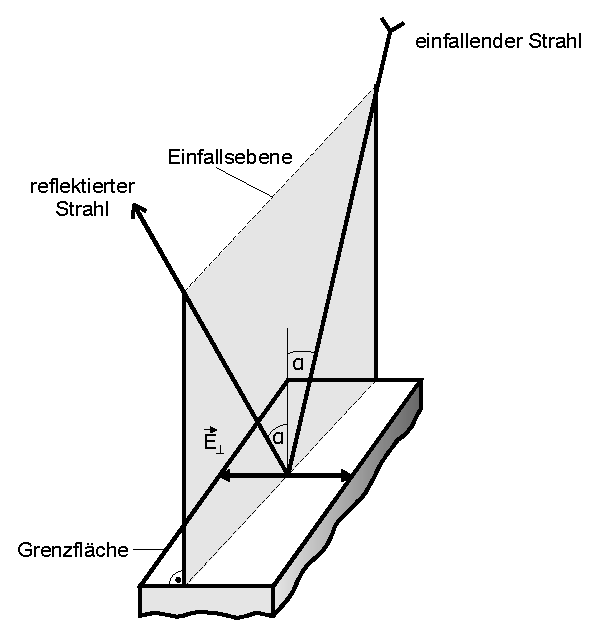
\includegraphics[height = 6cm]{sPol.pdf}
    \caption{Reflexion eines s-polarisierten Lichtstrahls an einer Grenzfläche \cite{ap407}.}
    \label{fig:sPol}
\end{figure}
Da das Linienintegral einer geschlossenen Kurve verschwindet, ist die Tangentialkomponente des Feldstärkevektors stetig. Daraus ergibt sich
\begin{equation*}
    \vec{E}_{\symup{e}_{\perp}} + \vec{E}_{\symup{r}_{\perp}} = \vec{E}_{\symup{d}_{\perp}} \; .
\end{equation*}
Aus dieser Stetigkeitsbedingung vereinfacht sich \autoref{eqn:strahlung3} zu 
\begin{equation*}
    \vec{E}_{\symup{r}_{\perp}} = - \vec{E}_{\symup{e}_{\perp}} \frac{\symup{ncos}\,\beta - \symup{cos}\,\alpha}{\symup{ncos}\,\beta + \symup{cos}\,\alpha} \; .
\end{equation*}
Mithilfe des Snelliusschen Brechungsgesetzes
\begin{equation*}
    \symup{n} = \frac{\symup{sin}\, \alpha}{\symup{sin}\, \beta}
\end{equation*}
erhält man die Fresnelschen Gleichungen 
\begin{equation*}
    \vec{E}_{\symup{r}_{\perp}} = - \vec{E}_{\symup{e}_{\perp}} \frac{\symup{sin}\left(\alpha - \beta\right)}{\symup{sin}\left(\alpha + \beta\right)}
\end{equation*}
und
\begin{equation}
    \vec{E}_{\symup{r}_{\perp}} = - \vec{E}_{\symup{e}_{\perp}} \frac{\left(\sqrt{\symup{n}^2-\symup{sin}^2 \, \alpha}-\symup{cos}\, \alpha\right)^2}{\symup{n}^2 - 1} \; .
    \label{eqn:fresnelS2}
\end{equation}
Wenn man \autoref{eqn:fresnelS2} nach n auflöst, erhält man
\begin{equation}
    n = \sqrt{1-\frac{4\vec{E}_{\symup{e}_{\perp}}\symup{cos}^2\, \alpha}{\left(\vec{E}_{\symup{r}_{\perp}}+\vec{E}_{\symup{e}_{\perp}}\right)^2}+\frac{4\vec{E}_{\symup{e}_{\perp}}\symup{cos}^2\, \alpha}{\vec{E}_{\symup{r}_{\perp}}+\vec{E}_{\symup{e}_{\perp}}}} \; .
    \label{eqn: n1}
\end{equation}

Nun wird die parallele Polarisationsrichtung betrachtet. Dabei schwingt $\vec{E}_{\|}$ in der Einfallsebene. Dies ist in \autoref{fig:pPol} dargestellt.
\begin{figure}
    \centering
    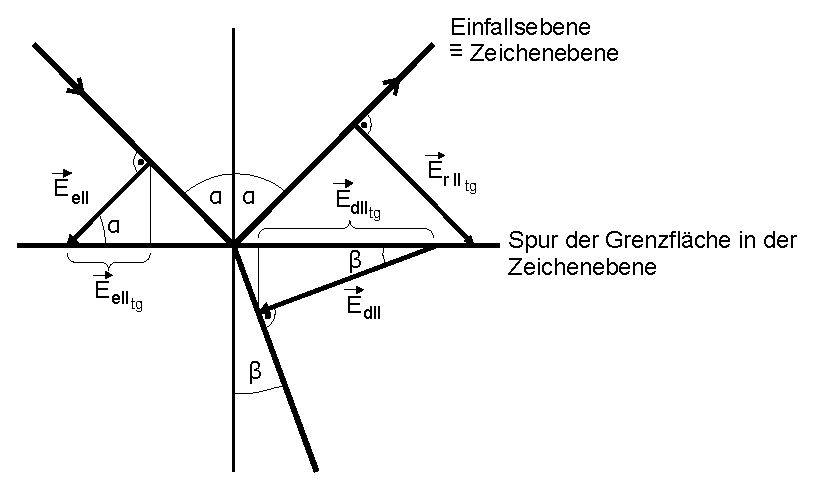
\includegraphics[height = 6cm]{pPol.pdf}
    \caption{Reflexion eines p-polarisierten Lichtstrahls an einer Grenzfläche \cite{ap407}.}
    \label{fig:pPol}
\end{figure}
$\vec{E}_{\|}$ besteht aus einer tangentialen Komponente $\vec{E}_{\| \symup{tg}}$ und einer normalen Komponente. Damit ergibt sich die Stetigkeitsbedingung 
\begin{equation*}
    \vec{E}_{\symup{e}\|\symup{tg}} + \vec{E}_{\symup{r}\|\symup{tg}} = \vec{E}_{\symup{d}\|\symup{tg}} \; .
\end{equation*}
Daraus folgt dann
\begin{equation*}
    \vec{E}_{\symup{r}\|} = \vec{E}_{\symup{e}\|} \frac{\symup{ncos}\, \alpha- \symup{cos}\, \beta}{\symup{ncos}\, \alpha + \symup{cos}\,\beta} \; .
\end{equation*}
Es ergeben sich mit dem Snelliusschen Brechungsgesetz weitere Fresnelsche Gleichungen
\begin{equation}
    \vec{E}_{\symup{r}\|} = - \vec{E}_{\symup{e}\|} \frac{\symup{tan}\left(\alpha - \beta\right)}{\symup{tan}\left(\alpha + \beta\right)}
    \label{eqn:fresnelP1}
\end{equation}
und
\begin{equation}
    \vec{E}_{\symup{r}\|} = \vec{E}_{\symup{e}\|}\frac{\symup{n}^2\symup{cos}\, \alpha - \sqrt{\symup{n}^2-\symup{sin}^2\,\alpha}}{\symup{n}^2\symup{cos}\, \alpha + \sqrt{\symup{n}^2-\symup{sin}^2\,\alpha}} \; .
    \label{eqn:fresnelP2}
\end{equation}
Auch diesmal kann \autoref{eqn:fresnelP2} nach n aufgelöst werden
\begin{equation*}
    n = \sqrt{\frac{1}{2}\left(\frac{\vec{E}_{\symup{r}\|}+\vec{E}_{\symup{e}\|}}{\vec{E}_{\symup{r}\|}-\vec{E}_{\symup{e}\|}}\frac{1}{\symup{cos}\,\alpha}\right)^2 \pm 
    \sqrt{\frac{1}{4}\left(\frac{\vec{E}_{\symup{r}\|}+\vec{E}_{\symup{e}\|}}{\vec{E}_{\symup{r}\|}-\vec{E}_{\symup{e}\|}}\frac{1}{\symup{cos}\,\alpha}\right)^4 - 
    \left(\frac{\vec{E}_{\symup{r}\|}+\vec{E}_{\symup{e}\|}}{\vec{E}_{\symup{r}\|}-\vec{E}_{\symup{e}\|}}\right)^2 \symup{tan}^2\, \alpha}} \; .
\end{equation*}
Mit \autoref{eqn:fresnelP1} wird $\vec{E}_{\symup{r}\|} = 0$ für $\alpha_{\symup{p}}+\beta_{\symup{p}} = 90°$. Mit dem Snelliusschen Brechungsgesetz
folgt dann für den Brewsterwinkel $\alpha_{\symup{p}}$
\begin{equation*}
    \symup{tan}\,\alpha_{\symup{p}} = \symup{n} \; . 
\end{equation*}
Der Brewsterwinkel beschreibt den Einfallswinkel, bei dem der Lichtstrahl nicht mehr reflektiert wird, sondern vollständig in das Medium eindringt.
\section{Aufbau}

\label{sec:Aufbau}
Benötigt werden ein Laser, in diesem speziellen Fall ein He-Ne-Laser, der mit Hilfe eines Polarisationsfilters polarisiert wird, ein Spiegel auf einem Goniometer, ein schwenkbares Photoelement, welches an einem Amperemeter angeschlossen wird. 
\begin{figure}
    \centering
    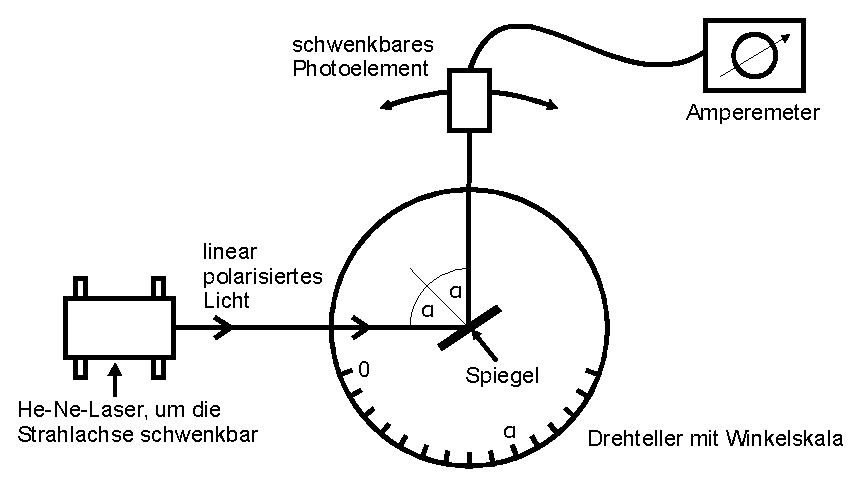
\includegraphics[height = 6cm]{GesamtAufbau.pdf}
    \caption{Aufbau der Messapparatur}
    \label{fig:GesamtAufbau}
\end{figure}
Der Aufbau ist in \autoref{fig:GesamtAufbau}schematisch dargestellt.

In \autoref{fig:AufbauKlein} ist die Drehplatte dargestellt.
\begin{figure}
    \centering
    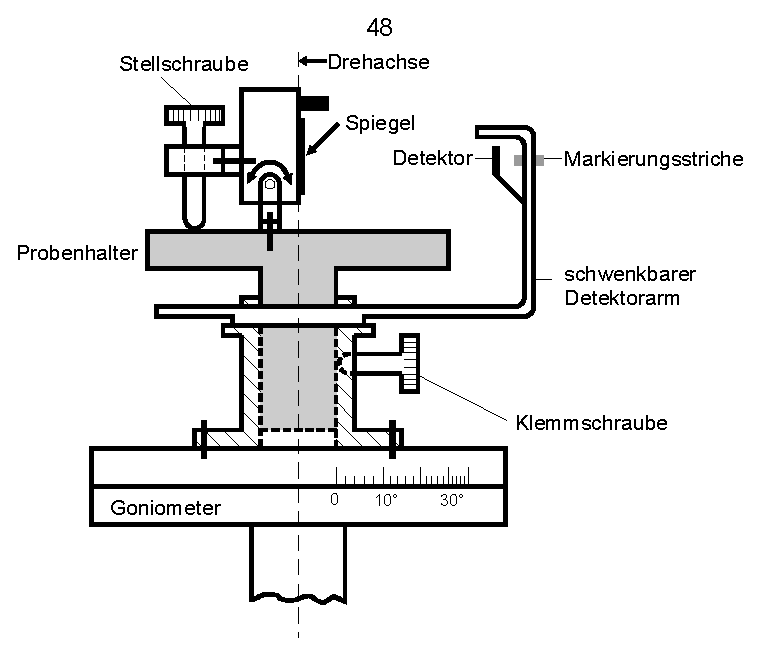
\includegraphics[height = 6cm]{AufbauKlein.pdf}
    \caption{Aufbau der Drehplattform}
    \label{fig:AufbauKlein}
\end{figure}
Auf dem Goniometer wird die Probenhalterung befestigt. AUf dieser wird der Spiegel mit einer Stellschraube befestigt. Unterhalb dieses Probenhalters wird der schwenkbare Detektorarm befestigt.

\section{Durchführung}
\label{sec:Durchführung}
Vor Beginn der Messung muss die Messapparatur justiert werden. Hierzu wird zunächst der Detektor so eingestellt,
dass der Laser exakt in dessen Öffnung strahlt. 
Nun muss der Filter eingesetzt werden, und es wir der Polarisationswinkel gemessen, unter welchem sich ein Minimum ergibt.
Im Anschluss muss dieser auf $0\unit{\degree}$ gestellt.
Danach wird der Spiegel eingesetzt, sodass die reflektierende Fläche senkrecht zum Leser steht.
Jetzt wird die Neigung des Spiegels so angepasst, dass die Reflexion des Lasers in dessen Öffnung strahlt, damit auch der Spiegel die exakte 
Höhe und Neigung hat.
Das Goniometer wird so justiert, dass ein zuverlässiges Ablesen möglich ist. Hierbei bietet sich an, die $0\unit{\degree}$-Marke in eine Reihe mit Laser und dem Spiegel zu stellen.
Jetzt werden Detektor und Spiegel so gedreht, dass die Reflexion des Spiegels bei kleinst möglichem Winkel in den Detektor trifft. Dieser Winkel liegt bei den verwendeten 
Bauteilen bei rund $6\unit{\degree}$.
Die gemessene Stromstärke wird notiert und der Winkel des Spiegels um $2\unit{\degree}$ erhöht. Dieser Vorgang muss so lange wiederholt werden bis keine Messung mehr Möglich ist ($\alpha <90\unit{\degree})$.
Die Messung wird für einen Polarisationswinkel $90\unit{\degree}$ analog durchgeführt.
\section{Auswertung}
\label{sec:Auswertung}

\subsection{Fehlerrechnung}
\label{sec:Fehlerrechnung}
Für die Fehlerrechnung werden folgende Formeln aus der Vorlesung verwendet.
für den Mittelwert gilt
\begin{equation}
    \overline{x}=\frac{1}{N}\sum_{i=1}^N x_i ß\; \;\text{mit der Anzahl N und den Messwerten x} 
    \label{eqn:Mittelwert}
\end{equation}
Der Fehler für den Mittelwert lässt sich gemäß
\begin{equation}
    \increment \overline{x}=\frac{1}{\sqrt{N}}\sqrt{\frac{1}{N-1}\sum_{i=1}^N(x_i-\overline{x})^2}
    \label{eqn:FehlerMittelwert}
\end{equation}
berechnen.
Wenn im weiteren Verlauf der Berechnung mit der fehlerhaften Größe gerechnet wird, kann der Fehler der folgenden Größe
mittels Gaußscher Fehlerfortpflanzung berechnet werden. Die Formel hierfür ist
\begin{equation}
    \increment f= \sqrt{\sum_{i=1}^N\left(\frac{\partial f}{\partial x_i}\right)^2\cdot(\increment x_i)^2}.
    \label{eqn:GaussMittelwert}
\end{equation}

\subsection{Bestimmung des Brechungsindex}
Es werden aus den Messungen zur parallelen und senkrechten Polarisation der Brechungsindex bestimmt. Zur Messung wurde ein Dunkelstrom 
$I_{\symup{D}} = 3\,\unit{\nano\ampere}$ gemessen. Dieser ist gegenüber der Messdaten vernachlässigbar klein.

\subsubsection{Senkrechte Polarisation}
Zuerst muss die gemessene Intensität umgerechnet werden. Es gilt
\begin{equation}
  \frac{I_{\symup{r}}}{I_{\symup{e}}} \thicksim \frac{E_{\symup{r}}^2}{E_{\symup{e}}^2} = E^2 \. .
    \label{eqn:energie}
\end{equation}
Dabei ist $I_e = 200 \, \unit{\micro\ampere}$. Die Messdaten zum Einfallswinkel, zur Intensität und zur Wurzel des Intensitätsverhältnisses 
$\frac{I_{\symup{r}}}{I_{\symup{e}}}$ sind in \autoref{tab:Pol0} dargestellt.
Des Weiteren wird mit \autoref{eqn: n1} und obiger Beziehung der Brechungsindex jeder einzelnen Messung berechnet und ebenfalls in \autoref{tab:Pol0} abgebildet.

\begin{table}
    \centering
    \caption{Messwerte der senkrechten Polarisation sowie der Brechungsindex n.}
    \begin{tabular}{c c c c}
        \toprule
        $\alpha \mathrm{/} \unit{\degree}$  & $I_{\symup{r}}\mathrm{/}\unit{\micro\ampere}$ & $\frac{I_{\symup{r}}}{I_{\symup{e}}}$ & n\\
        \midrule
        6&67&0.5788&3.6098 \\
        8&70&0.5916&1.1403 \\
       10&66&0.5745&3.1518 \\
       12&72&0.6000&3.4178 \\
       14&67&0.5788&1.1153 \\
       16&70&0.5916&3.7433 \\
       18&73&0.6042&2.7793 \\
       20&76&0.6164&1.9471 \\
       22&78&0.6245&4.3261 \\
       24&72&0.6000&1.9233 \\
       26&80&0.6325&2.9728 \\
       28&74&0.6083&3.9614 \\
       30&80&0.6325&1.2023 \\
       32&80&0.6325&3.7460 \\
       34&82&0.6403&3.9058 \\
       36&84&0.6481&1.1588 \\
       38&85&0.6519&4.5423 \\
       40&90&0.6708&3.4662 \\
       42&92&0.6782&2.2786 \\
       44&93&0.6819&5.2867 \\
       \bottomrule
    \end{tabular}
    \quad
    \begin{tabular}{c c c c}
        \toprule
        $\alpha \mathrm{/} \unit{\degree}$  & $I_{\symup{r}}\mathrm{/}\unit{\micro\ampere}$ & $\frac{I_{\symup{r}}}{I_{\symup{e}}}$ & n\\
        \midrule
       46&97&0.6964&2.5779 \\
       48&99&0.7036&3.7581 \\
      50&100&0.7071&5.6304 \\
      52&100&0.7071&1.3696 \\
      54&100&0.7071&4.8658 \\
      56&100&0.7071&5.0002 \\
      58&100&0.7071&1.2117 \\
      60&100&0.7071&5.5594 \\
      62&100&0.7071&3.9945 \\
      64&110&0.7416&2.7970 \\
      66&120&0.7746&7.8703 \\
      68&120&0.7746&3.5797 \\
      70&120&0.7746&5.0458 \\
      72&130&0.8062&9.0196 \\
      74&140&0.8367&2.1677 \\
      76&140&0.8367&9.2864 \\
      78&140&0.8367&9.6592 \\
      80&140&0.8367&1.5901 \\
     82&160&0.8944&17.0442 \\
     84&160&0.8944&12.2245 \\
        \bottomrule
    \end{tabular}
    \label{tab:Pol0}
\end{table}

Der gemittelte Brechungsindex ergibt sich zu $\symup{n} = 4.3482$.

\subsubsection{parallele Polarisation}
Erneut wird die Intensität mittels \autoref{eqn:energie} umgerechnet. Dabei ist $I_e = 140 \, \unit{\micro\ampere}$. Die Messwerte sind in 
\autoref{tab:Pol90} dargestellt.
\begin{table}
    \centering
    \caption{Messwerte der parallelen Polarisation sowie der Brechungsindex n.}
    \begin{tabular}{c c c c}
        \toprule
        $\alpha \mathrm{/} \unit{\degree}$  & $I_{\symup{r}}\mathrm{/}\unit{\micro\ampere}$ & $\frac{I_{\symup{r}}}{I_{\symup{e}}}$ & n\\
        \midrule
        6&54.0&0.6211&4.4499 \\
        8&54.0&0.6211&29.3909 \\
        10&54.0&0.6211&5.0803 \\
        12&53.0&0.6153&4.9574 \\
       14&52.0&0.6094&30.1278 \\
        16&50.0&0.5976&4.1396 \\
        18&50.0&0.5976&5.9831 \\
        20&50.0&0.5976&9.7023 \\
        22&49.0&0.5916&3.8974 \\
        24&48.0&0.5855&8.9898 \\
        26&45.0&0.5669&5.5596 \\
        28&44.0&0.5606&3.6834 \\
       30&44.0&0.5606&23.0123 \\
        32&43.0&0.5542&4.1554 \\
        34&41.0&0.5412&3.9350 \\
       36&37.0&0.5141&24.3370 \\
        38&39.0&0.5278&3.3791 \\
        40&38.0&0.5210&4.7218 \\
        42&36.0&0.5071&7.6073 \\
        44&34.0&0.4928&2.9437 \\
       \bottomrule
    \end{tabular}
    \quad
    \begin{tabular}{c c c c}
        \toprule
        $\alpha \mathrm{/} \unit{\degree}$  & $I_{\symup{r}}\mathrm{/}\unit{\micro\ampere}$ & $\frac{I_{\symup{r}}}{I_{\symup{e}}}$ & n\\
        \midrule
        46&32.0&0.4781&6.5104 \\
        48&30.0&0.4629&4.2061 \\
        50&29.0&0.4551&2.7589 \\
       52&26.0&0.4309&15.4058 \\
        54&22.0&0.3964&2.7481 \\
        56&22.0&0.3964&2.6743 \\
       58&20.0&0.3780&18.5681 \\
        60&17.0&0.3485&2.1569 \\
        62&14.0&0.3162&2.7803 \\
        64&10.0&0.2673&4.3344 \\
         66&8.0&0.2390&1.6287 \\
         68&6.7&0.2188&3.4441 \\
         70&4.6&0.1813&2.1495 \\
         72&2.5&0.1336&1.3309 \\
         74&1.4&0.1000&7.0543 \\
         76&1.0&0.0845&1.3069 \\
         78&2.0&0.1195&1.3886 \\
        80&5.2&0.1927&13.3533 \\
        82&12.0&0.2928&1.9046 \\
        84&22.0&0.3964&3.3430 \\
        86&46.0&0.5732&9.5785 \\
        \bottomrule
    \end{tabular}
    \label{tab:Pol90}
\end{table}
Der Brechungsindex berechnet sich dabei über \autoref{eqn:n90} und wird ebenfalls in der Tabelle dargestellt. 
Der Mittelwert der Brechungsindizes ergibt sich so zu $\bar{n}= 7.4670$.

Außerdem lässt sich mittels der Messung zur parallelen Polarisation der Brewsterwinkel bestimmen. Dieser befindet sich beim Minimum der 
reflektierten Intensität und liegt somit bei $\alpha_{\symup{p}} = 76°$. Mittels \autoref{eqn:brewster} berechnet sich der Brechungsindex somit zu  
$\symup{n} = 4.0107$.

\subsection{Plot der Messwerte und Vergleich mit der Theorie}
Um die Theoriekurven darstellen zu können wird erneut der Mittelwert der gemittelten Brechungsindizes bestimmt. Dabei wird jedoch der durch die Messung
der parallelen Polarisation bestimmte Brechungsindex $\bar{n}= 7.4670$ aus der Mittelung ausgenommen, da die Abweichung zu den anderen beiden gemittelten
Brechungsindizes zu groß ist.  Damit ergibt sich ein Brechungsindex von
$\bar{\symup{n}} = 4.1795$.

In \autoref{fig:plot0} wird nun $\sqrt{I/I_0}$ gegen den Einfallswinkel $\alpha$ aufgetragen. Die Theoriekurve berechnet sich durch \autoref{eqn:fresnelS2}. 
\begin{figure}
    \centering
    \includegraphics[height = 10cm]{build/plot0Pol.pdf}
    \caption{Vergleich der Messwerte mit der Theorie der senkrechten Polarisation.}
    \label{fig:plot0}
\end{figure}

In \autoref{fig:plot90} wird $\sqrt{I/I_0}$ der parallelen Polarisation gegen den Einfallswinkel $\alpha$ aufgetragen. Die Theoriekurve berechnet sich diesmal 
durch \autoref{eqn:fresnelP2}.
\begin{figure}
    \centering
    \includegraphics[height = 10cm]{build/plot90Pol.pdf}
    \caption{Vergleich der Messwerte mit der Theorie der parallelen Polarisation.}
    \label{fig:plot90}
\end{figure}
\section{Diskussion}
\label{sec:Diskussion}

In den beiden graphischen Darstellungen \autoref{fig:plot0} und \autoref{fig:plot90} ist zusehen, dass die Messwerte relativ nah an der Theoriekurve liegen. 
Der Brechungsgindex der über die beiden Polarisationsrichtung und den Brewsterwinkel bestimmt wurde, unterscheiden sich jedoch deutlicher von dem Theoriewert $n_{\text{theo}}=3.353$. Mit
experimentell bestimmten Werten von $\bar{n}=7.4670$, $\bar{n}= 4.0107$ und $\bar{n}= 4.1795$ liegt die Abweichung zum Theoriewert bei $122.7\%$,  $19.6\%$ bzw. $24.7\%$. Eine mögliche Ursache dafür kann neben der teilweise geringen
Genauigkeit beim Ablesen auch an möglichen Ungenauigkeiten beim Drehen der Vorrichtung entstanden sein. So konnte beim Rotieren des Spiegels und des Detektors auch geringes ein Mitdrehen des Goniometers nicht gänzlich ausgeschlossen werden.
Hinzukommen veränderliche Lichtverhältnisse, die einen Einfluss auf die Messung des Photoelements gehabt haben könnten. Diese Fehlerquelle war trotz eines vorheringen Bestimmens des Dunkelstroms nicht vollständig zu eliminieren.

Zusammenfassend kann also festgehalten werden, dass trotz der Bemühungen eine möglichst genaue Messreihe aufzunehmen, einige Fehler und Ungenauigkeiten nur minimiert, nicht aber ausgeschlossen werden konnten.

\newpage
\printbibliography
\nocite{ap407}
\nocite{matplotlib}
\nocite{numpy}
\nocite{scipy}
\nocite{uncertainties}
\nocite{reback2020pandas}

\newpage
%\includepdf[scale=0.9,pages=1,pagecommand=\section*{Anhang}\thispagestyle{empty}]{messdaten.pdf}
%\addcontentsline{toc}{section}{\protect\numberline{}Anhang}
%\includepdf[scale=0.9,pages=2-]{messdaten.pdf}
%\includepdf[pages=-]{messdaten.pdf}

\end{document}
